% exercise sheet with header on every page for math or close subjects
\documentclass[12pt]{article}
\usepackage[utf8]{inputenc} 
\usepackage{latexsym} 
\usepackage{multicol}
\usepackage{fancyhdr}
\usepackage{amsfonts} 
\usepackage{amsmath}
\usepackage{amssymb}
\usepackage{enumerate}
\usepackage{listings}
\usepackage{graphicx}
\usepackage{pdfpages}

% Shortcuts for bb, frak and cal letters
\newcommand{\E}{\mathbb{E}}
\newcommand{\V}{\mathbb{V}}
\renewcommand{\P}{\mathbb{P}}
\newcommand{\N}{\mathbb{N}}
\newcommand{\R}{\mathbb{R}}
\newcommand{\C}{\mathbb{C}}
\newcommand{\Z}{\mathbb{Z}}
\newcommand{\Pfrak}{\mathfrak{P}}
\newcommand{\Pfrac}{\mathfrak{P}}
\newcommand{\Bfrac}{\mathfrak{P}}
\newcommand{\Bfrak}{\mathfrak{B}}
\newcommand{\Fcal}{\mathcal{F}}
\newcommand{\Ycal}{\mathcal{Y}}
\newcommand{\Bcal}{\mathcal{B}}
\newcommand{\Acal}{\mathcal{A}}

% formating
\topmargin -1.5cm 
\textheight 24cm
\textwidth 16.0 cm 
\oddsidemargin -0.1cm

% Fancy Header on every Page
\pagestyle{fancy}
\lhead{\textbf{Programmierung for Engineers - Exercise 3}}
\rhead{Daniel Schäfer (2549458)\\ Dominik Weber (2548553)\\ Sina Vaghiri (2533563)}
\renewcommand{\headrulewidth}{1.2pt}
\setlength{\headheight}{60pt} 

\begin{document}
\pagenumbering{gobble}
\lstset{language=C}

\section{Messreihen}
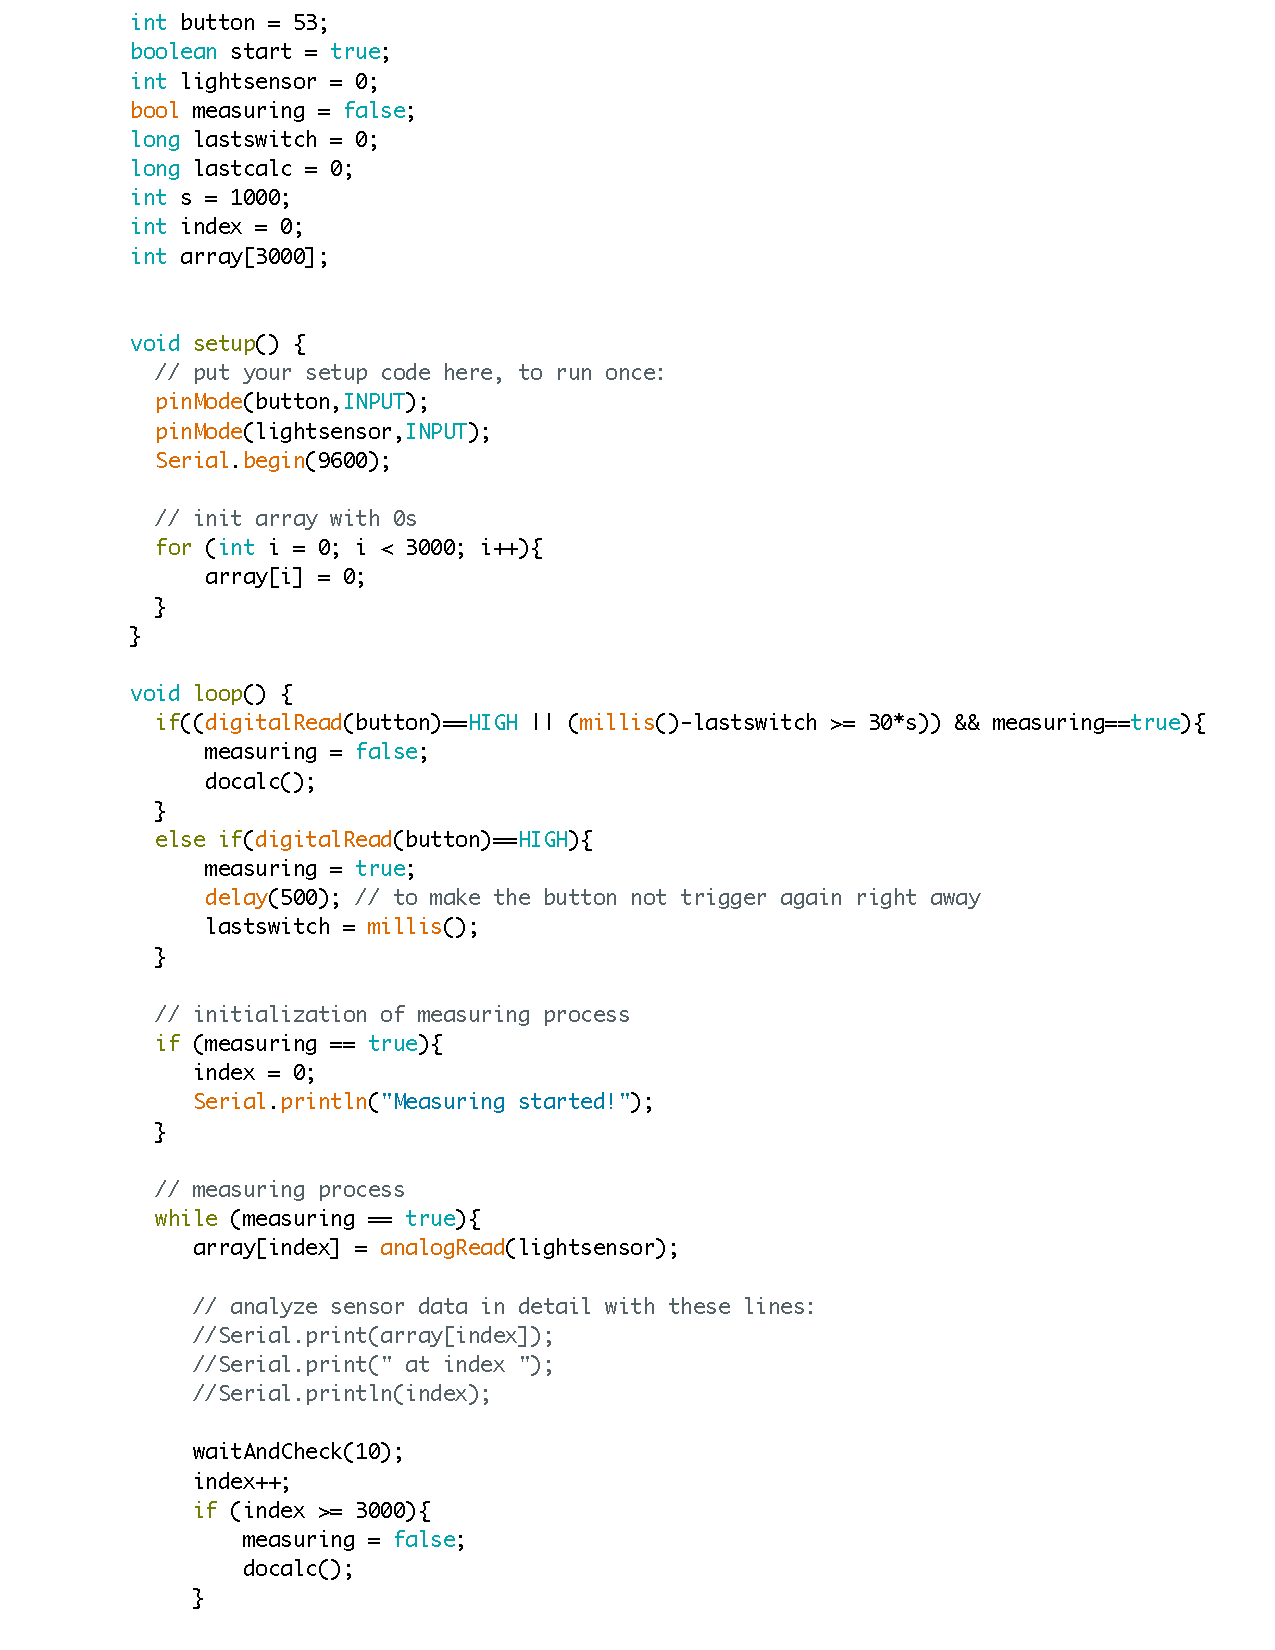
\includepdf[pages=-]{../Aufgabe1/Aufgabe1.pdf}

\section{Senso}
\subsection{Die Implementierung}
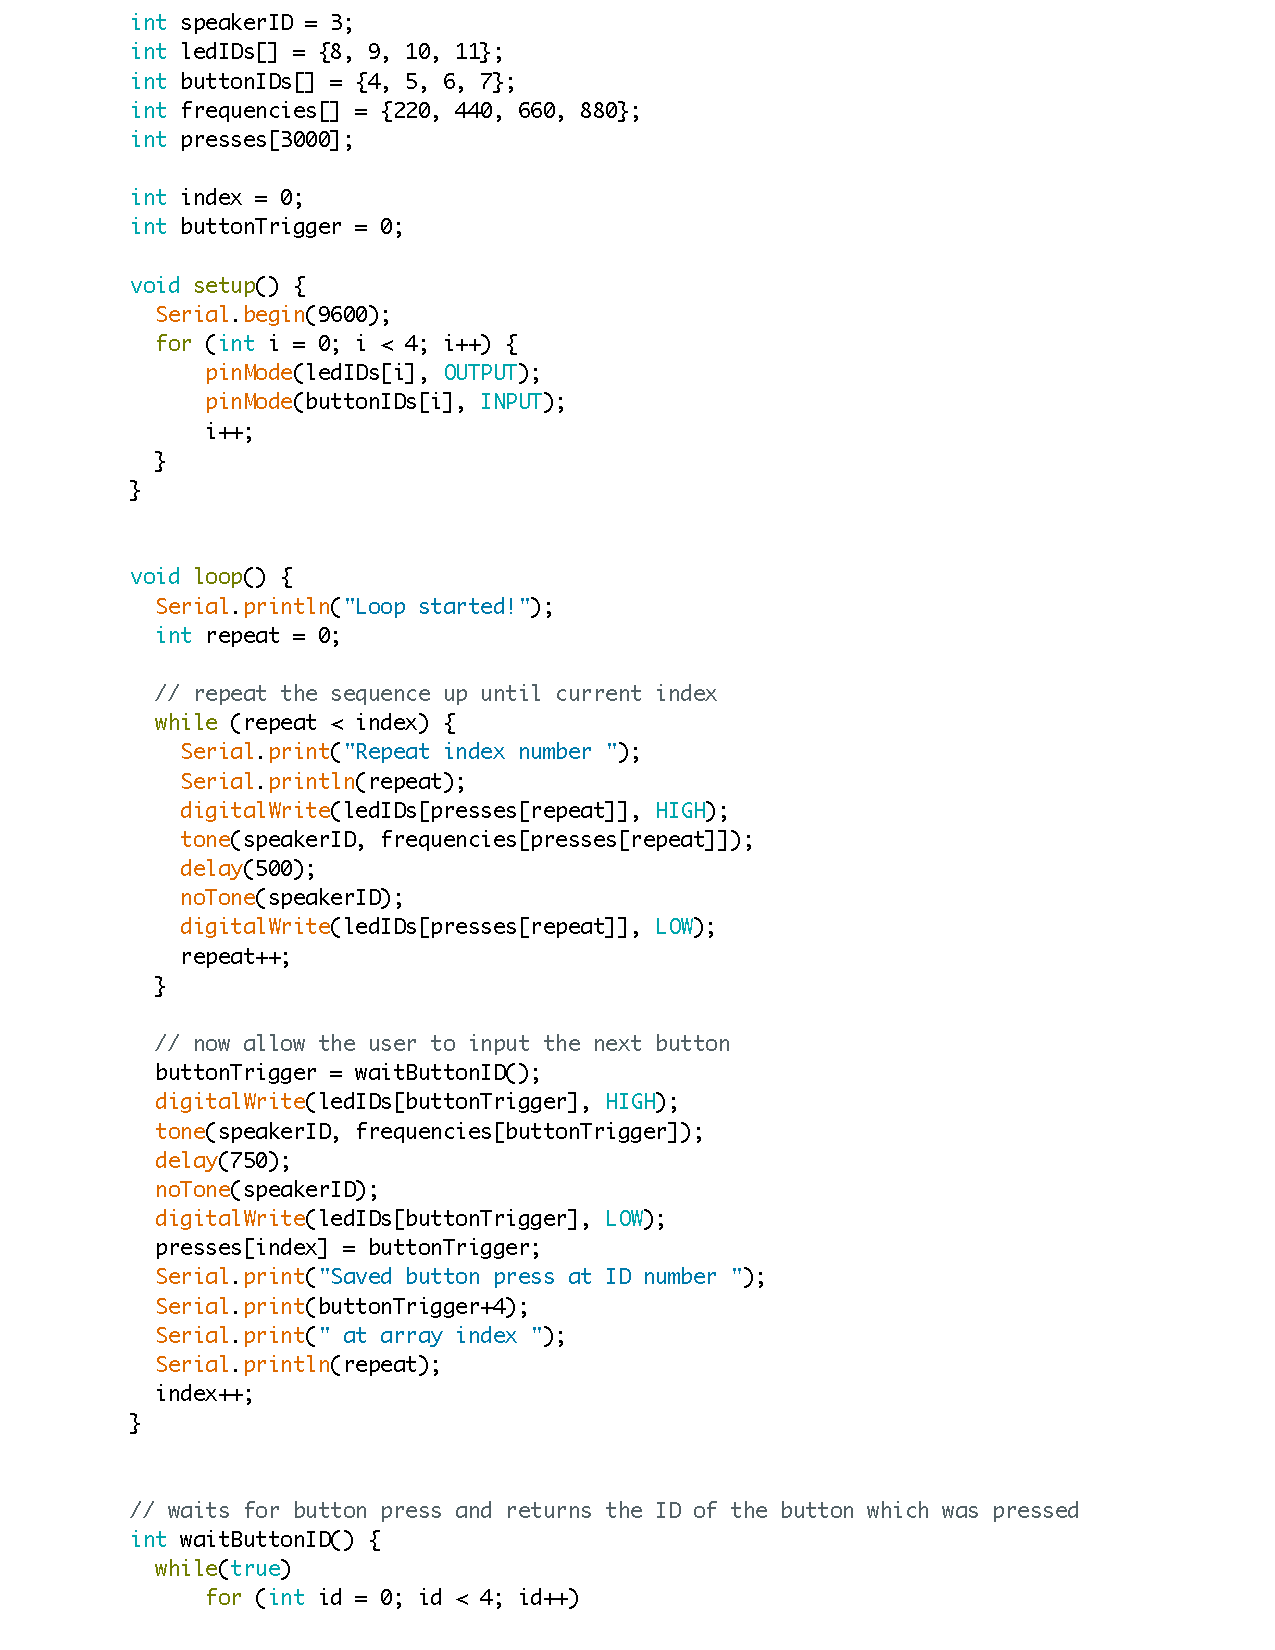
\includepdf[pages=-]{../Aufgabe2/Aufgabe2.pdf}

\subsection{Arraygroesse}
We will reach out of bounds if we capture over 3000 presses. So we should either use an implementation like in 2.3 because we can't create an array with unlimited (or undefined) size or we should use a different datastructure instead of arrays (linked list would be a nice fit for this specific task) but obviously you will still be limited by the amount of memory available.

\subsection{Bonus: Ringspeicher}
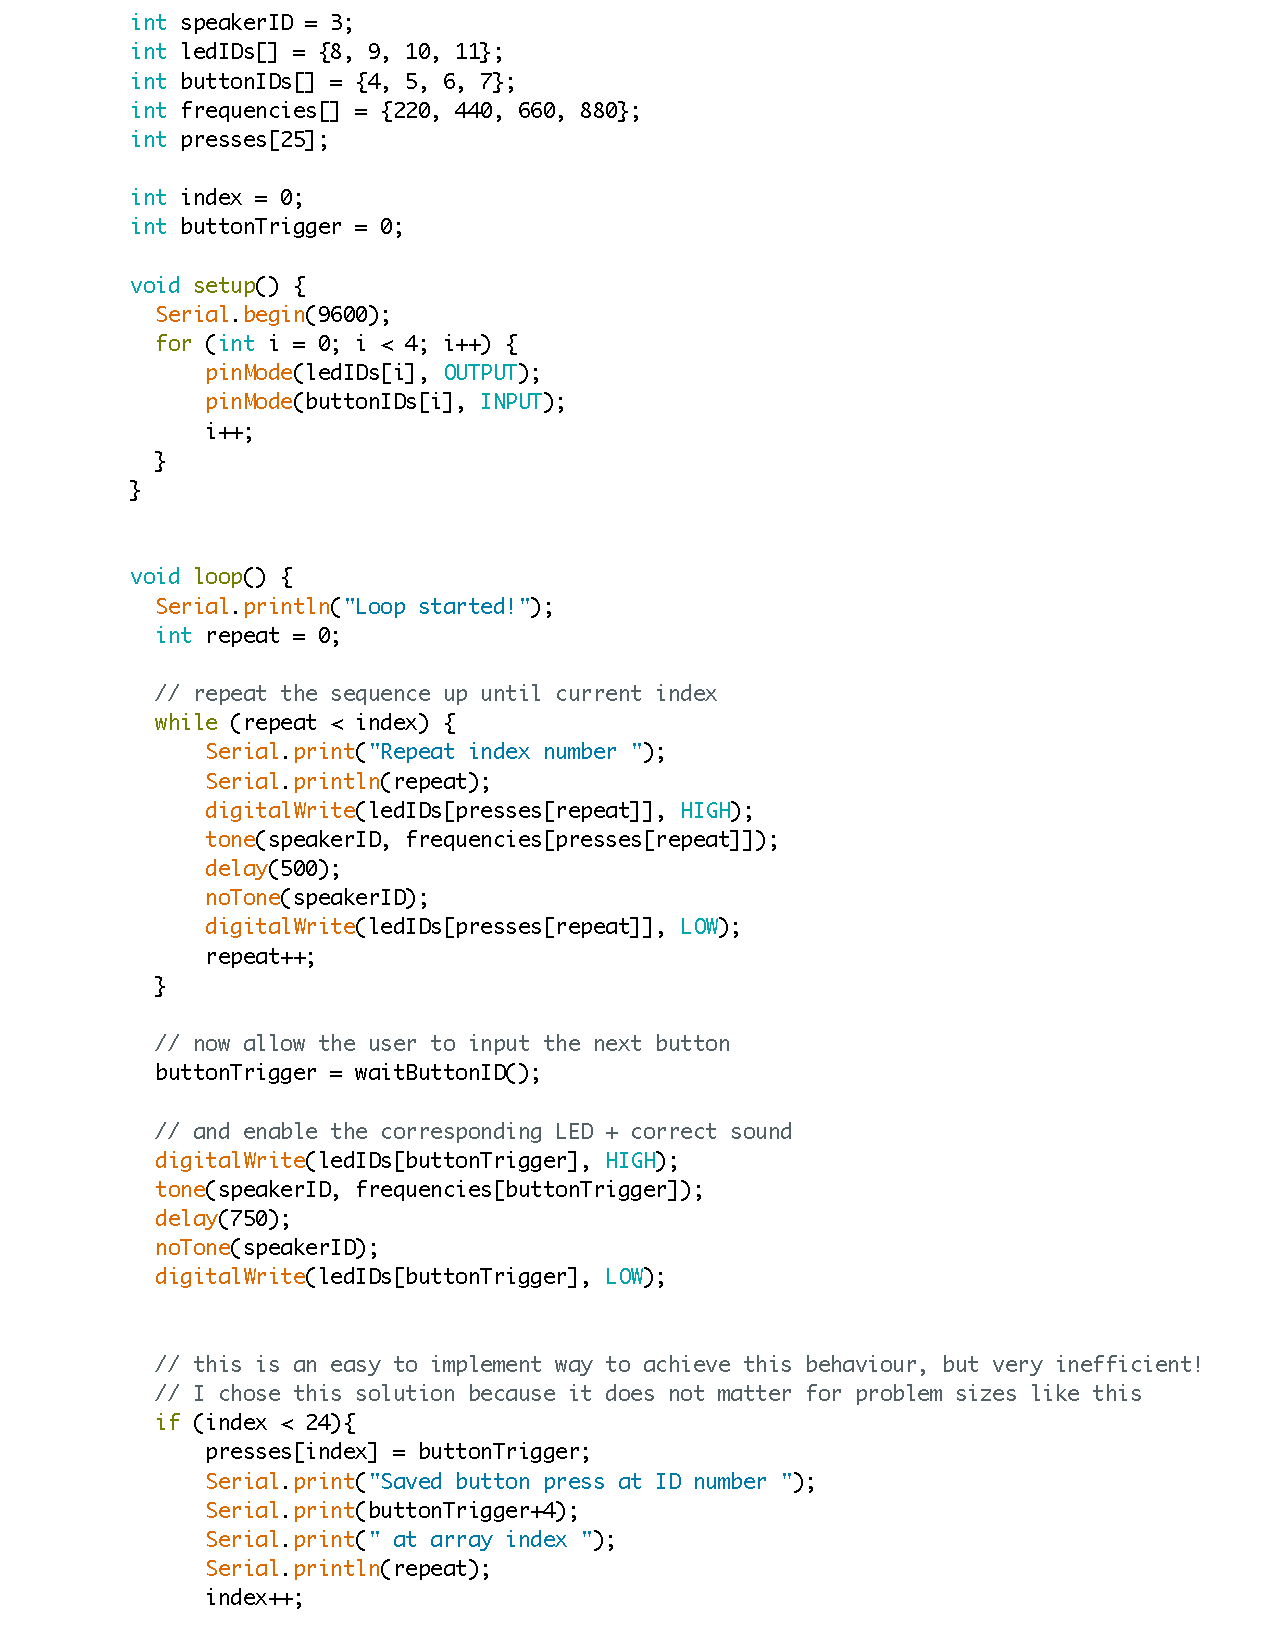
\includepdf[pages=-]{../Aufgabe23/Aufgabe23.pdf}


\end{document}
